Via de simples calculs d'aires, il est très facile de découvrir les classiques identités remarquables
$(a + b)^2 = a^2 + b^2 + 2ab$,
$(a - b)^2 = a^2 + b^2 - 2ab$
et
$(a + b)(a - b) = a^2 - b^2$.
%
Par exemple, en considérant le dessin ci-dessous où $ABCD$, $AEGF$ et $GHCK$ sont des carrés,
il est évident que $(a + b)^2 = a^2 + b^2 + 2 ab$.
Malheureusement, cette démonstration n'est valable que pour $a > 0$ et $b > 0$ \emph{(ce sont des contraintes géométriques concrètes)}.

\begin{center}
	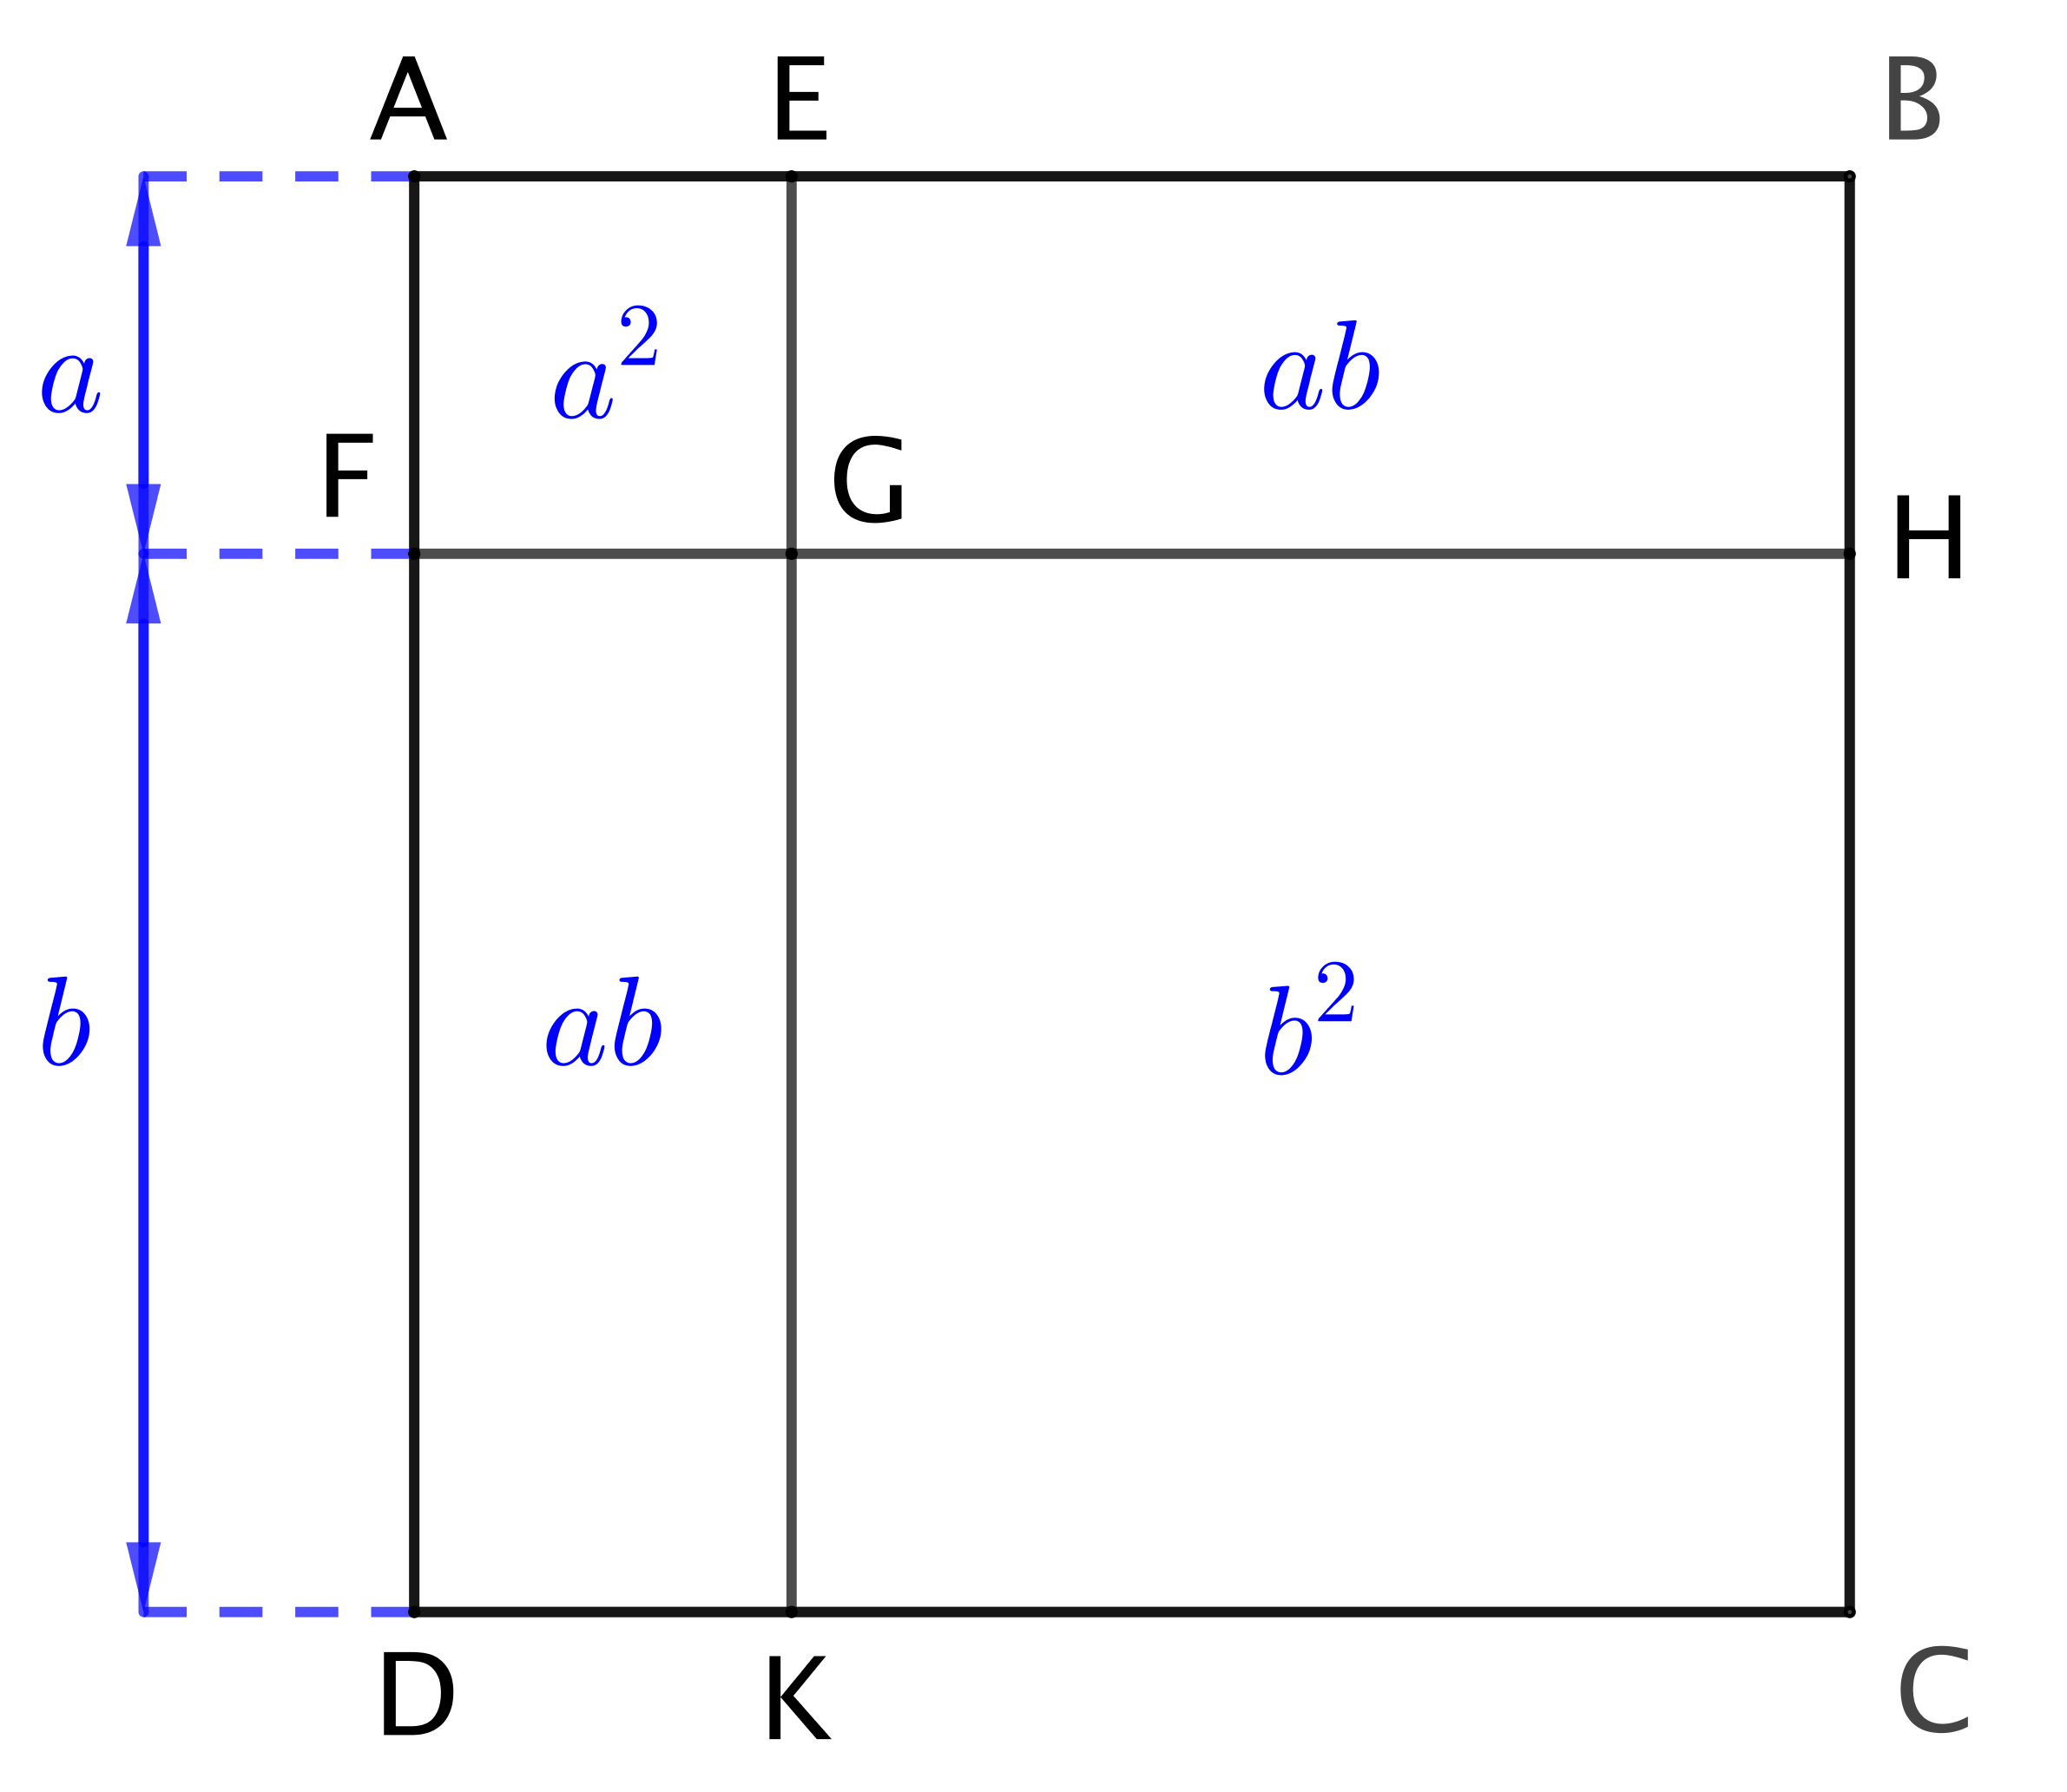
\includegraphics[scale = .7]{(a+b)^2.png}
\end{center}


Comment passer à $(a + b)^2 = a^2 + b^2 + 2 ab$ pour $a$ et $b$ deux complexes de signes quelconques ?
Classiquement, une vérification est faite via un calcul algébrique.
%
En résumé, nous conjecturons géométriquement, puis nous validons algébriquement.
%
Bien que rigoureuse, la démarche précédente est peu satisfaisante, car elle balaye d'un revers de main l'approche géométrique, dont le rôle est réduit à la découverte d'une formule.
Si nous considérons le dessin ci-après, il est dommage de devoir faire du calcul algébrique pour valider $(a + b + c)^2 = a^2 + b^2 + c^2 + 2 ab + 2 ac + 2 bc$ pour $a$, $b$ et $c$ des complexes de signes quelconques.
Ce serait bien de pouvoir passer directement à l'identité pour $a$, $b$ et $c$ de signes quelconques.
Nous allons voir que cela est possible

\begin{center}
	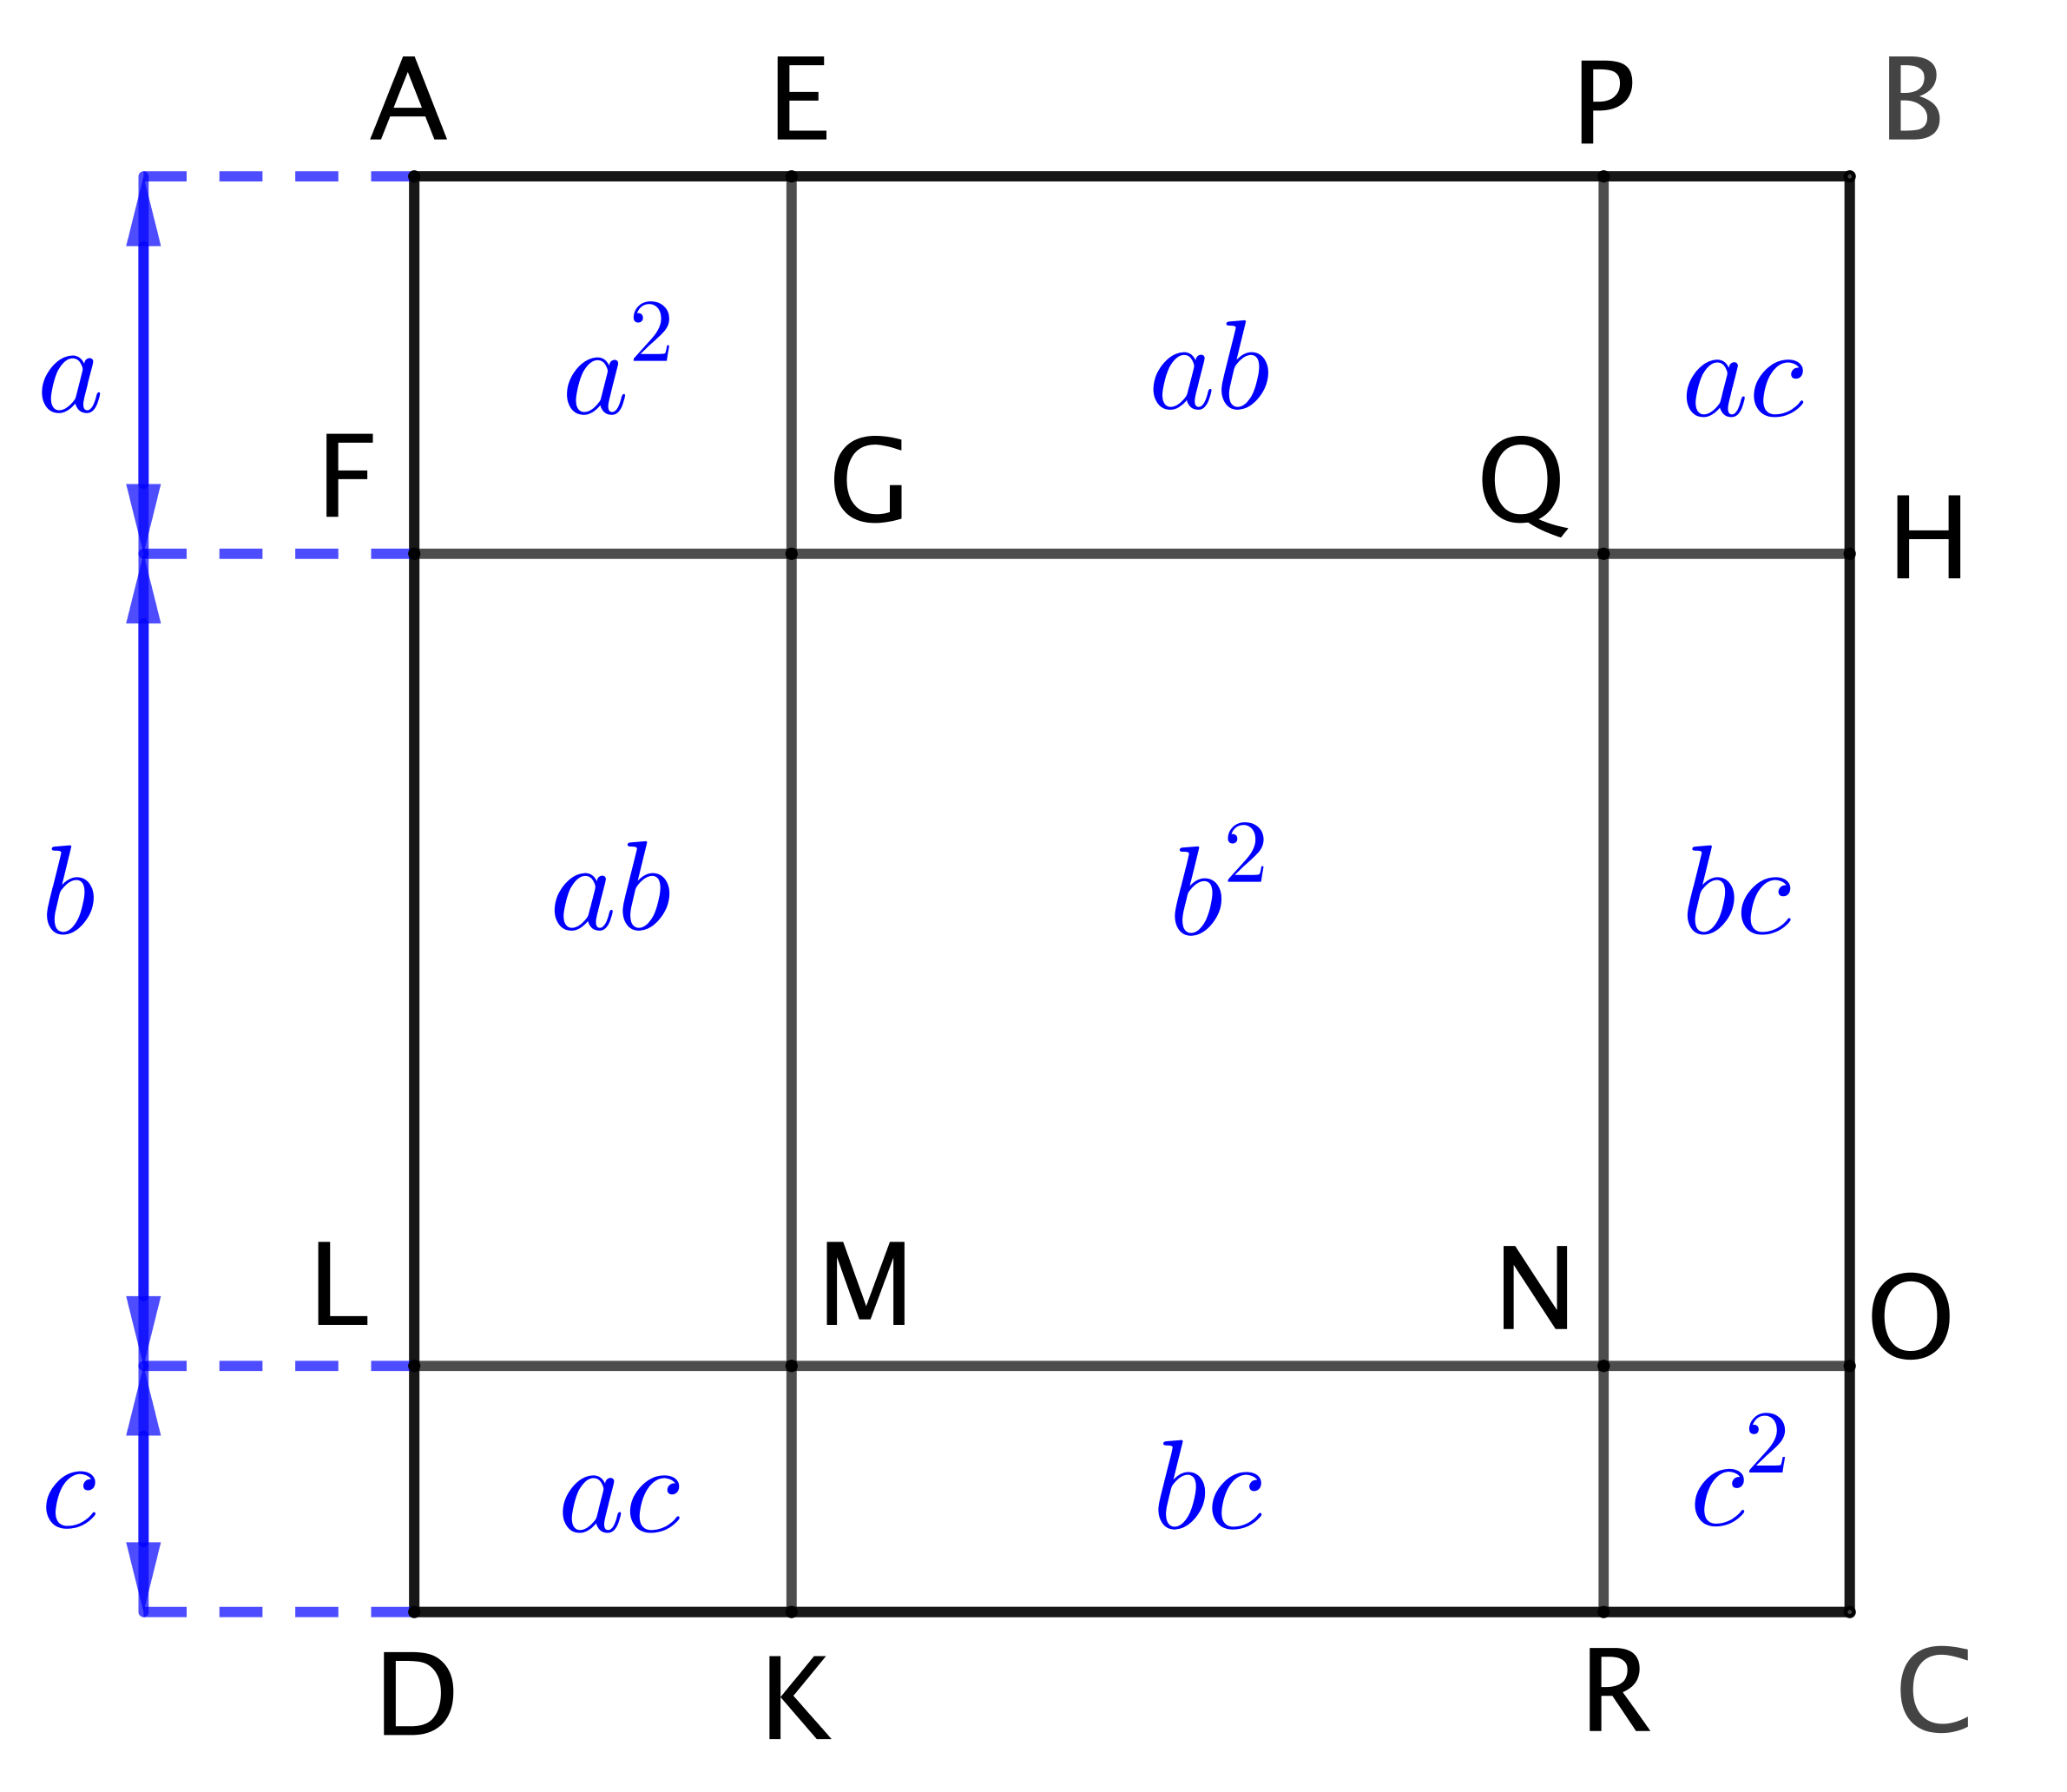
\includegraphics[scale = .7]{(a+b+c)^2.png}
\end{center}


% ----------- %


\begin{preli} \label{poly-finite-zeros}
	Si $p: \CC \rightarrow \CC$ est une fonction polynomiale de degré $n \in \NNs$,
	alors $\forall \lambda \in \CC$,
	il existe une fonction polynomiale $q(x)$ de degré $(n-1)$ vérifiant
	$p(x) - p(\lambda) = (x - \lambda) q(x)$.
	Ceci implique que $p$ ne peut pas avoir plus de $n$ zéros.
\end{preli}


\newpage
\begin{proof}
	Posant $p(x) = \sum_{k=0}^{n} a_k x^k$ avec $a_n \neq 0$ par hypothèse, nous avons:
	
	\begin{stepcalc}[style=sar]
	    p(x) - p(\lambda)
	\explnext{}
	    \dsum_{k=0}^{n} a_k (x^k - \lambda^k)
	\explnext{}
	    \dsum_{k=1}^{n} a_k (x - \lambda) \big( \sum_{i=0}^{k-1} x^i \lambda^{k-1-i} \big)
	\explnext{}
	    (x - \lambda) \dsum_{k=1}^{n} \dsum_{i=0}^{k-1} a_k x^i \lambda^{k-1-i} 
	\end{stepcalc}
	
	La factorisation conjointe à la diminution du degré ne permet pas d'avoir plus de $n$ zéros. 
\end{proof}


% ----------- %


\begin{fact} \label{poly-nullity-pos}
	Soit $p: \CC^n \rightarrow \CC$ une fonction polynomiale, où $n \in \NNs$.
	Si $p$ s'annule sur $\big( \RRsp \big)^n$, alors $p$ s'annule sur $\CC^n$ tout entier. 
\end{fact}


\begin{proof}
	Raisonnons par récurrence sur $n \in \NNs$ pour démontrer la validité de la propriété $\setproba{P}(n)$ définie par
	\emph{\og 
		Pour toute fonction polynomiale $p: \CC^n \rightarrow \CC$,
		si $p$ s'annule sur $\big( \RRsp \big)^n$,
		alors $p$ s'annule sur $\CC^n$ tout entier. 
	\fg}\kern2pt.
	%
	\begin{itemize}[label=\small\textbullet]
		\item \textbf{Cas de base.}
		%
		$\setproba{P}(1)$ signifie qu'une fonction polynomiale à une variable s'annulant sur $\RRsp$ est identiquement nulle sur $\CC$ tout entier.
		%
		Or, selon le \refpreli{poly-finite-zeros}, un polynôme complexe non nul n'a qu'un nombre fini de racines, donc $\setproba{P}(1)$ est validée.


		\item \textbf{Hérédité.}
		%
		Supposons $\setproba{P}(n)$ valide pour $n \in \NNs$.
		Soit $p$ une fonction polynomiale à $(n + 1)$ variables vérifiant les conditions de la propriété $\setproba{P}(n + 1)$.
		%
		\begin{enumerate}
		    \item Pour $\alpha \in \RRsp$ fixé,
		    posons $p_\alpha(x_1 ; ... ; x_n) = p(x_1 ; ... ; x_n ; \alpha)$.
		    Nous savons que $p_\alpha$ vérifie les conditions de la propriété $\setproba{P}(n)$,
		    donc par hypothèse de récurrence, nous avons:
		    $\forall (x_1 ; ... ; x_n) \in \CC^n$,
		    $p_\alpha(x_1 ; ... ; x_n) = 0$,
		    soit $p(x_1 ; ... ; x_n ; \alpha) = 0$.


		    \item Pour $x_1$ , ... , $x_n$ des complexes quelconques,
		    posons $\ell(x) = p(x_1 ; ... ; x_n ; x)$.
		    Le point précédent montre que $\ell$ vérifie $\setproba{P}(1)$, donc, d'après le cas de base,
		    $\forall x \in \CC$,
		    $\ell(x) = 0$,
		    soit $p(x_1 ; ... ; x_n ; x) = 0$.


		    \item Finalement,
		    $\forall (x_1 ; ... ; x_n ; x) \in \CC^{n+1}$,
		    $p(x_1 ; ... ; x_n ; x) = 0$.
		    Autrement dit, nous avons déduit la validité de $\setproba{P}(n+1)$ à partir de celle de $\setproba{P}(n)$.
		\end{enumerate}
		
		
		\item \textbf{Conclusion.}
		%
		Par récurrence sur $n \in \NNs$, la propriété $\setproba{P}(n)$ est vraie pour tout naturel non nul $n$.
	\end{itemize}

	\null\vspace{-6ex}
\end{proof}


% ----------- %


\begin{example}
    Si nous reprenons les deux dessins initiaux, le \reffact{poly-nullity-pos} précédent rend licite le passage des formules géométriques contraintes au cas général en faisant les choix suivants de fonctions polynomiales.
    %
    \begin{itemize}[label=\small\textbullet]
    	\item $p_1(a ; b) = (a + b)^2 - a^2 - b^2 - 2 ab$
    
    	\item $p_2(a ; b ; c) = (a + b + c)^2 - a^2 - b^2 - c^2 - 2 ab - 2 ac - 2 bc$
    \end{itemize}
\end{example}
% ----------- %


\begin{example}
	En utilisant une approche géométrique semblable à celle présentée plus haut avec une diagonale de carrés, il devient évident, et rigoureux maintenant, que $\forall n \in \NNs$, $\forall (a_1 ; ... ; a_n) \in \CC^n$, nous avons:
    %
    \[
    	\big( \dsum_{k=1}^{n}a_k \big)^2
    	=
    	\dsum_{k=1}^{n} \left( a_k \right)^2
    	+
    	2 \dsum_{1 \leq i < j \leq n} a_i a_j
    \]
\end{example}


% ----------- %


\begin{example}
	Nous laissons le soin au lecteur de vérifier à l'aide d'un cube, le solide géométrique, la validité de l'identité $(a + b)^3 = a^3 + 3 a^2 b + 3 a b^2 + b^3$ sur $\CC^2$.
\end{example}


% ----------- %


\newpage
Considérons maintenant le dessin ci-dessous avec la contrainte $a > b$.
%
\begin{center}
	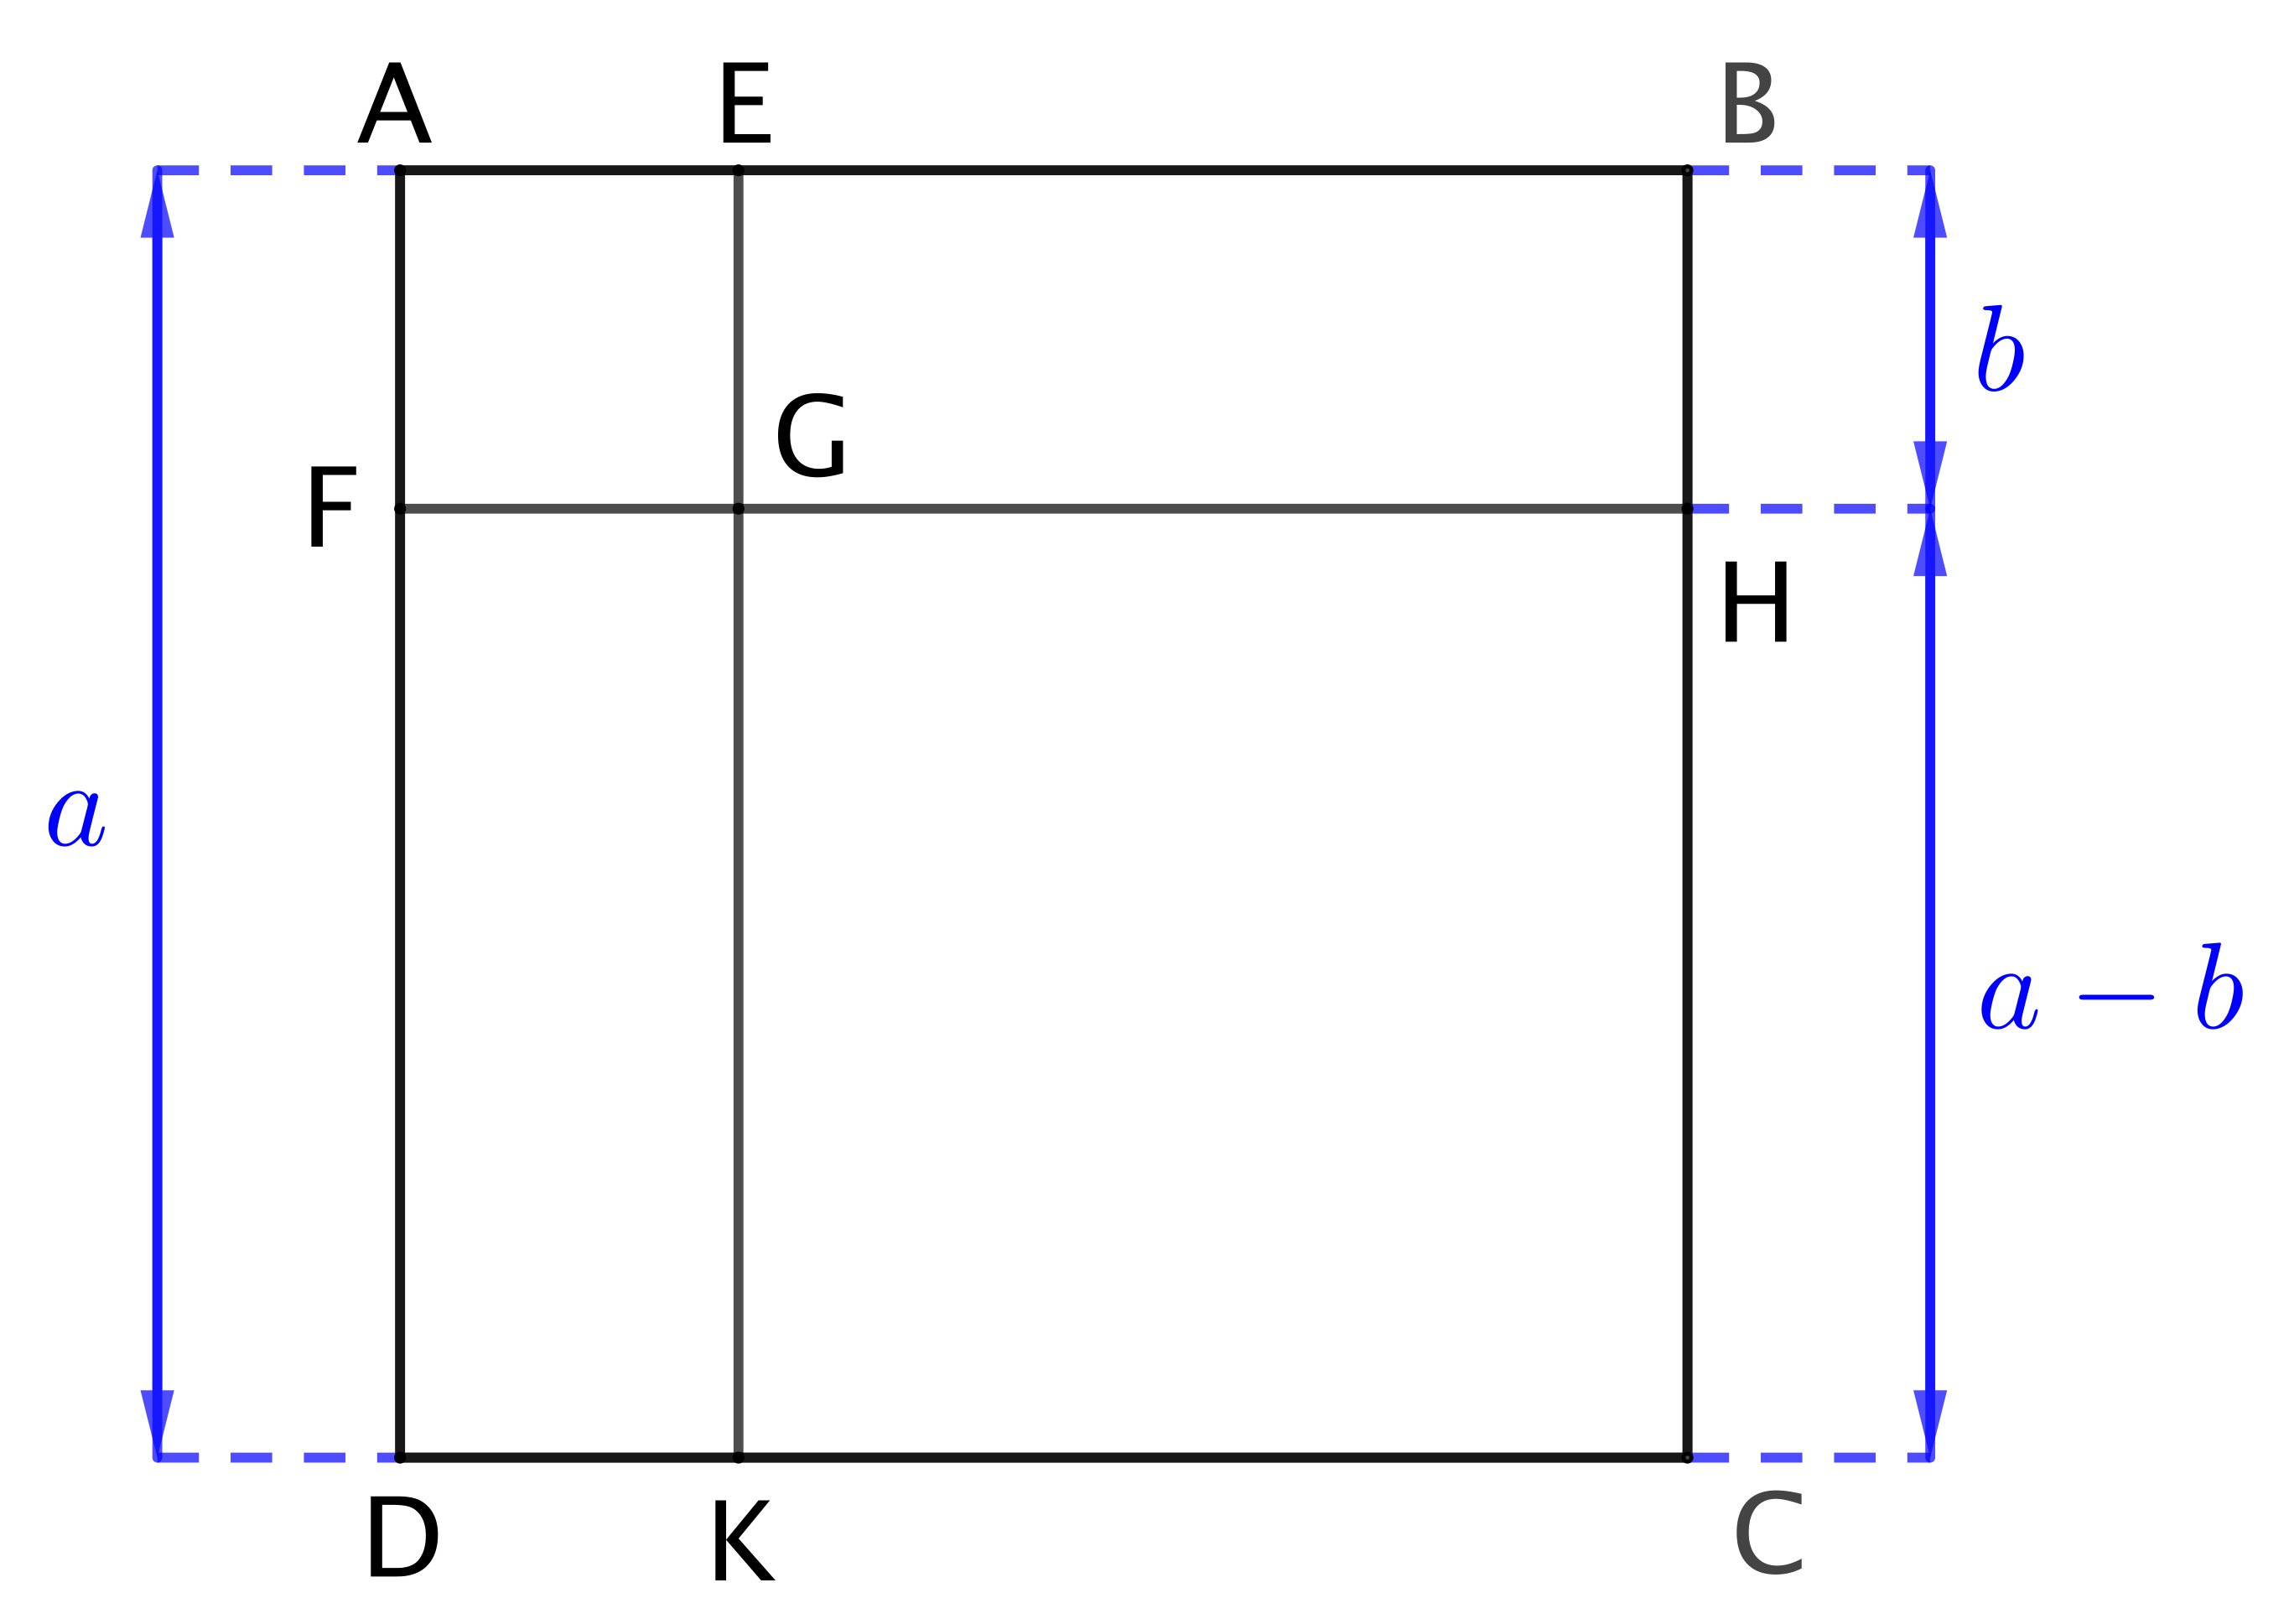
\includegraphics[scale = .7]{(a-b)^2.png}
\end{center}

Le \reffact{poly-nullity-pos} ne peut pas s'appliquer au calcul géométrique évident suivant.

\smallskip
\leavevmode\kern-1em%
\begin{stepcalc}[style=ar*, ope={\iff}]
    \area{GHCK} = \area{ABCD} - \area{ABHF} - \area{AEKD} + \area{AEGF}
\explnext{}
    (a-b)^2 = a^2 - 2ab + b^2
\end{stepcalc}
\smallskip

Peut-on tout de même déduire du calcul géométrique précédent la validité sur $\CC^2$ de l'identité $(a - b)^2 = a^2 + b^2 - 2ab$?
Cela est rendu possible par le \reffact{poly-nullity-interval} suivant. 


\medskip

\begin{fact} \label{poly-nullity-interval}
	Soit $p: \CC^n \rightarrow \CC$ une fonction polynomiale, où $n \in \NNs$.
	Si $p$ s'annule sur $\setgeo*{E}{1} \times \cdots \times \setgeo*{E}{n}$ où chaque $\setgeo*{E}{k} \subseteq \CC$ est infini,
	alors $p$ s'annule sur $\CC^n$ tout entier. 
\end{fact}


\begin{proof}
	Il suffit d'adapter la preuve du \reffact{poly-nullity-pos}
	(se souvenir que la clé du raisonnement était l'impossibilité, pour une fonction polynomiale, d'avoir une infinité de racines).
\end{proof}


% ----------- %


\medskip

\begin{example}
	En reprenant le dessin précédent, nous avons les calculs géométriques simples suivants, toujours avec la contrainte $a > b$.

	\smallskip
	\leavevmode\kern-1em%
	\begin{stepcalc}[style=ar*, ope={\iff}]
    	\area{ABCD} - \area{AEGF} = \area{GHCK} + \area{EBHG} + \area{FGKD}
	\explnext{}
    	a^2 - b^2 = \area{GHCK} + \area{EBHG} + \area{FGKD}
	\end{stepcalc}
	\smallskip

	En déplaçant ensuite le rectangle $EBHG$ comme ci-dessous, nous obtenons alors un rectangle de dimension $(a+b) \times (a-b)$. 

	\begin{center}
		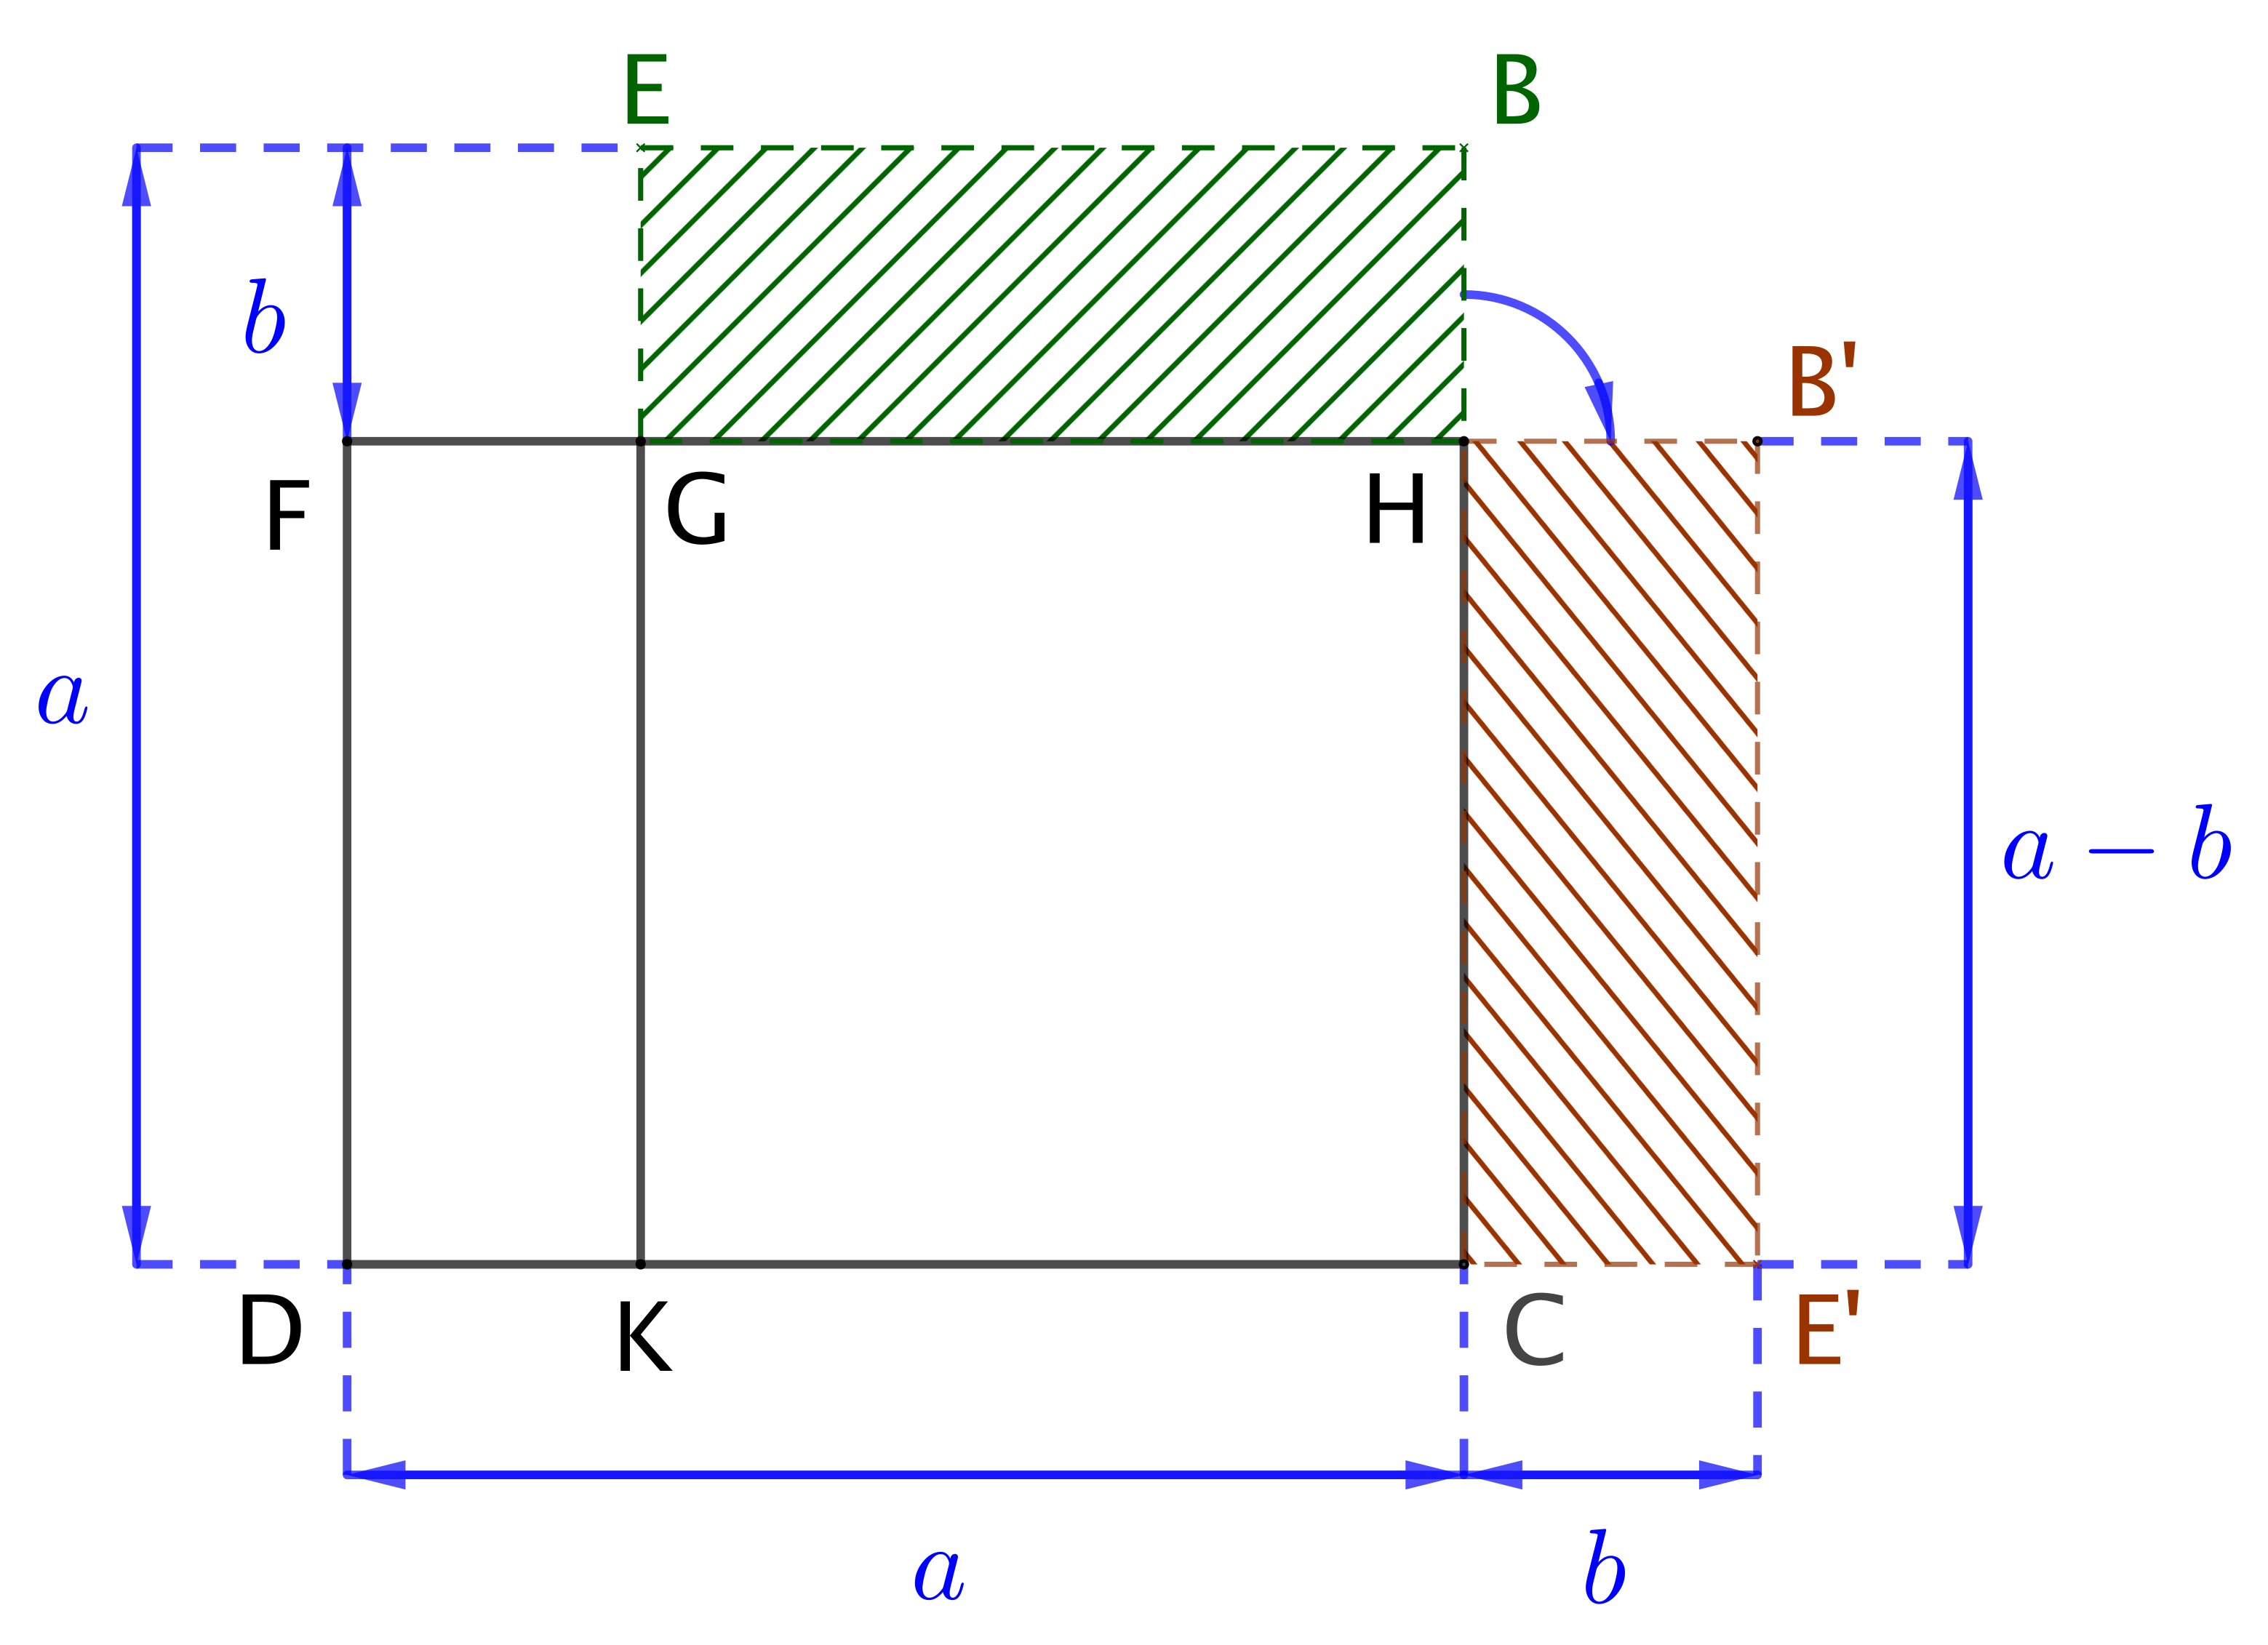
\includegraphics[scale = .7]{a^2-b^2.png}
	\end{center}

	Finalement, nous obtenons $a^2 - b^2 = (a+b)(a-b)$ si $a > b$,
	puis,
	en appliquant le \reffact{poly-nullity-interval} au polynôme $p(a ; b) = a^2 - b^2 - (a+b)(a-b)$,
	nous avons:
	$\forall (a ; b) \in \CC^2$, $a^2 - b^2 = (a+b)(a-b)$.
\end{example}


% ----------- %


\begin{example}
    Via le dessin suivant, sous les contraintes géométriques
    $\widetilde{\mathtt{u}} > \mathtt{u}$
    et
    $\widetilde{\mathtt{v}} > \mathtt{v}$,
    nous obtenons sans effort l'identité polynomiale
    $ \widetilde{\mathtt{u}} \widetilde{\mathtt{v}}
    - \mathtt{u} \mathtt{v}
    = \mathtt{v} ( \widetilde{\mathtt{u}} - \mathtt{u} )
    + \widetilde{\mathtt{u}} ( \widetilde{\mathtt{v}} - \mathtt{v} )$
    sur $\CC^2$ tout entier.

	\begin{center}
		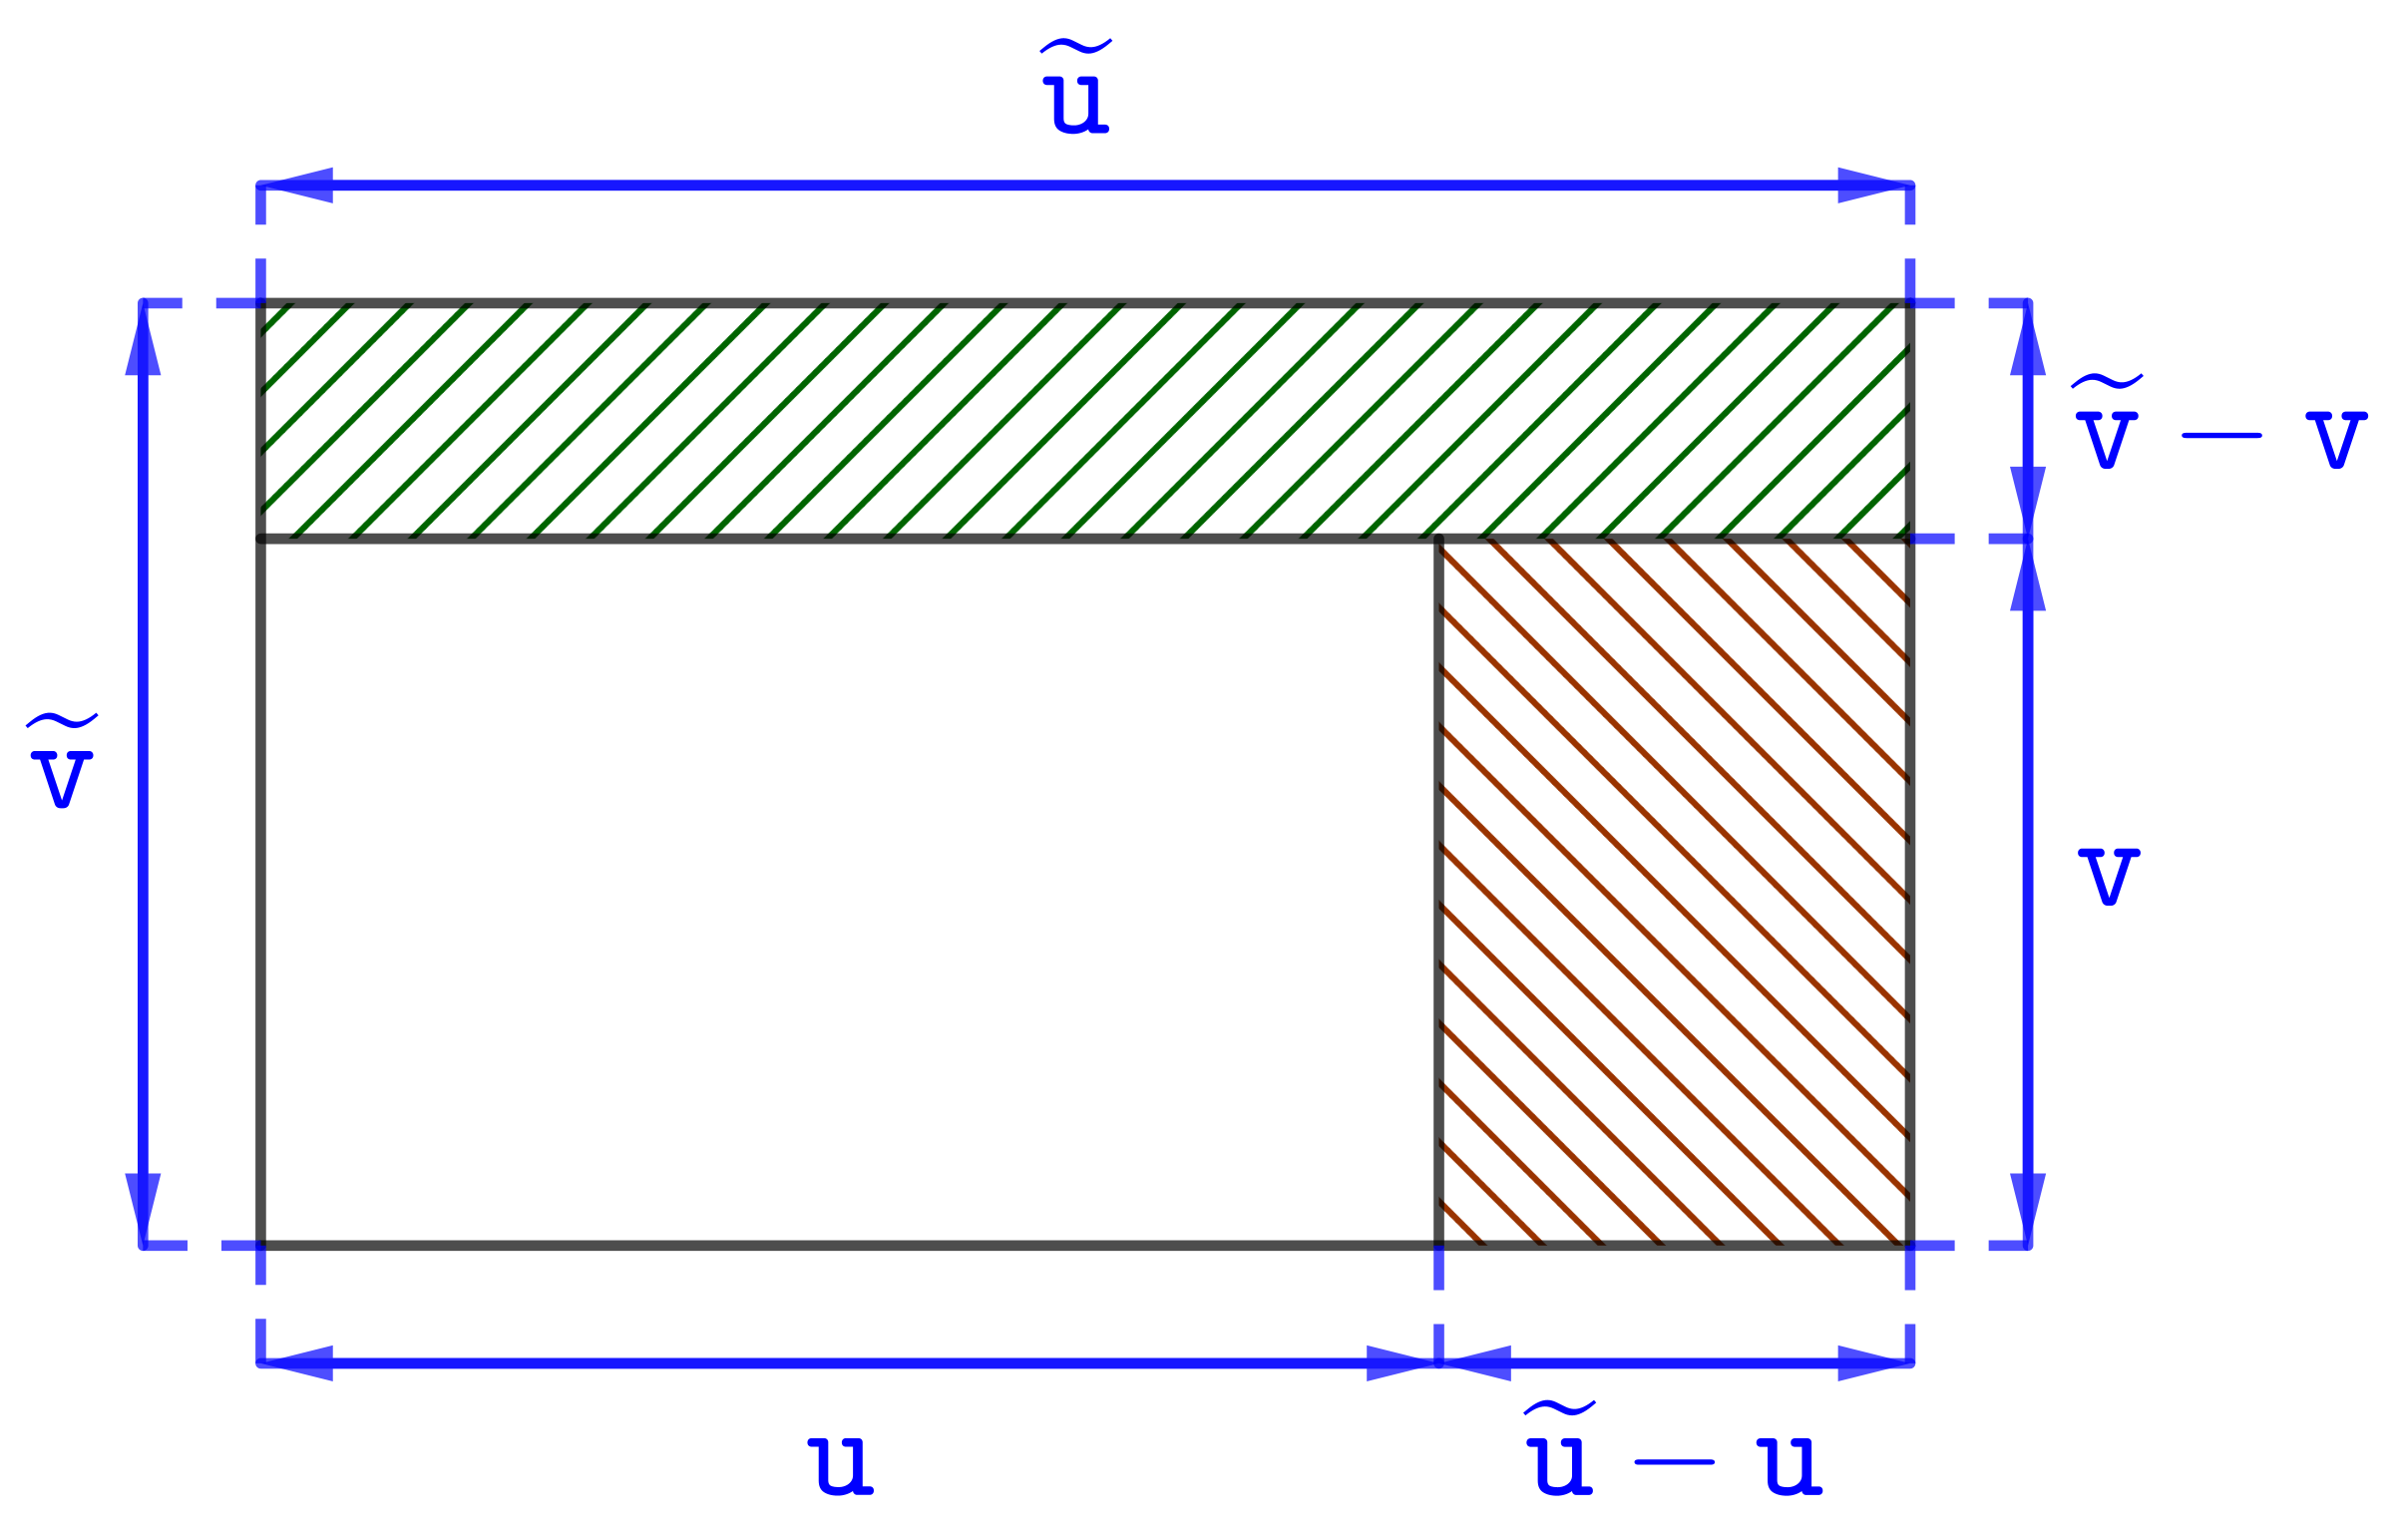
\includegraphics[scale=.75]{proder.png}
	\end{center}
    
    L'identité précédente rend naturelle la démonstration de la dérivabilité du produit de deux fonctions via l'égalité ci-dessous.
    %
    \[
          \frac{u(a+h) v(a+h) - u(a) v(a)}{h}
        = \frac{v(a) \big( u(a+h) - u(a) \big)}{h} 
        + \frac{u(a+h) \big( v(a+h) - v(a) \big)}{h}
    \]
\end{example}
